% !TeX encoding=utf8
% !TeX spellcheck = de-CH

%%% --- title based on maketitle --- --- --- ---

% \subject{Master thesis \\ University <insert>}
% \title{<insert title>}
% \author{<insert author>}
% \date{<insert date>}
% \maketitle


%%% --- title for this template --- --- --- ---

\begin{titlepage}
	\mbox{}\vspace{5\baselineskip}\\
	\rmfamily\huge
	\centering
	\textsc{Evaluierung der Retrieval-Leistung einer Search Engine am Beispiel der Bibel} \\
	
	% \mbox{}\vspace{1\baselineskip}\\
	\vspace{2em}
	Michael Hadorn\\
	\vspace{\baselineskip}
	\rmfamily\Large
	\today\\
	Version \input{version.txt}\mbox{} \\
	\normalsize
	
	\vspace{7em}
	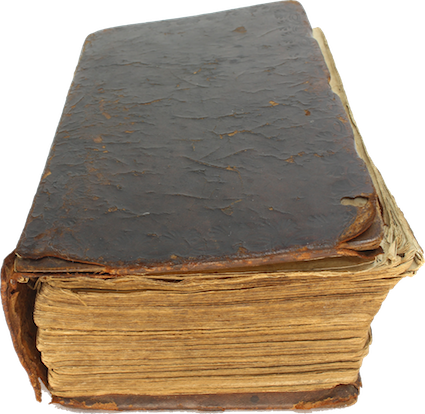
\includegraphics[width=0.25\textwidth]{images/0-title/bible.png}
	
	\vfill

	\begin{center}
		\begin{tabular}[h]{ r l }
			\textsc{\small{Studiengang}} & Informatik 8 BA 2012\\
			\textsc{\small{Seminararbeit}} & 2016\\
			\textsc{\small{Dozentin}} & Dr. Ruxandra Domenig\\
			\textsc{\small{Schule}} & ZHAW - School of Engineering\\
		\end{tabular}
	\end{center}

\end{titlepage}
